\setcounter{section}{50}
\section{B-дерево: определение и практическая значимость.}
\par \textbf{Определение:} \textit{B-дерево} - сильноветвистое сбалансированное дерево поиска, в каждом узле которого находится массив ключей, упорядоченных по убыванию. Между любыми двумя ключами находится "стрелка" на уровень ниже, значения всех элементов этого поддерева лежат между значениями этих ключей (см. рисунок). У дерева есть параметр $t \geqslant 2, t \in \mathbb{Z}$.
\begin{figure} [h]
    \centering
    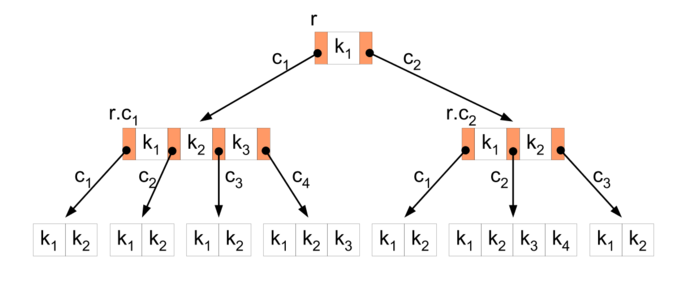
\includegraphics[scale=0.5]{images/51-54_b tree}
\end{figure}
\par B-дерево обладает следующими свойствами
\begin{enumerate}
    \item Каждый узел, кроме корня, содержит не менее $t - 1$ ключей, и каждый внутренний узел имеет по меньшей мере $t$ дочерних узлов. Если дерево не является пустым, корень должен содержать как минимум один ключ. 
    \item Каждый узел, кроме корня, содержит не более $2t - 1$ ключей и не более чем $2t$ сыновей во внутренних узлах
    \item Корень содержит от $1$ до $2t - 1$ ключей, если дерево не пусто и от $2$ до $2t$ детей при высоте большей $0$.
    \item Каждый узел дерева, кроме листьев, содержащий ключи $k_1, \ldots, k_n$, имеет $n + 1$ сына. $i$-й сын содержит ключи из отрезка $[k_{i - 1}; k_i],\:  k_0 = -\infty,\: k_{n + 1} = \infty$.
    \item Ключи в каждом узле упорядочены по неубыванию.
    \item Все листья находятся на одном уровне.
\end{enumerate}
\par \textbf{Практическая значимость:} Переходы в рамках массива осуществляются быстрее чем по указателям на листья, так как элементы массива лежат в одной области памяти. Поэтому структура B-дерева применяется для организации индексов во многих современных СУБД.
\\

\section{Оценка глубины B-дерева при фиксированном параметре t.}
\par \textbf{Утверждение:} Если в B-дереве всего $n$ ключей, то его глубина есть $O(\log_t n)$
\par $\blacktriangle$ Построим самое глубокое дерево из возможных. Тогда в каждой его вершине содержится минимальное возможное количество ключей (то есть в корневой вершине: 1 ключ, в остальных: $t-1$ ключ). Тогда на корневом уровне - 1 ключ, на первом - $2(t-1)$, на втором - $2t(t-1)$ (у каждой вершины t детей) ..., на $h$-ом - $2t^{h-1}(t-1)$.
\par Общее количество ключей: $1+2(t-1)+2t(t-1)+\ldots+2t^{h-1}(t-1)=n$
$$2(t-1)(1+t+t^2+\ldots+t^{h-1})=n-1$$
$$2(t-1)\frac{t^h-1}{t-1}=n-1 \text{ (собрали сумму геометрической прогрессии)}$$
$$t^h-1=\frac{n-1}{2}$$
$$t^h=\frac{n+1}{2}$$
$$h=\log_t \frac{n+1}{2}=O(\log_t n) \quad \blacksquare$$
\setcounter{section}{52}
\section{Реализация операции insert в B-дереве.}
\par Ищем лист, в который можно добавить ключ, совершая проход от корня к листьям. Если найденный узел не заполнен, добавляем в него ключ. Иначе разбиваем узел на два узла, в первый добавляем первые $t - 1$ ключей, во второй — последние $t - 1$ ключей. Оставшийся средний элемент добавляется в родительский узел, где становится разделительной точкой для двух новых поддеревьев (см. рисунок). После добавляем ключ в один из этих узлов.
\begin{figure}[h]
    \centering
    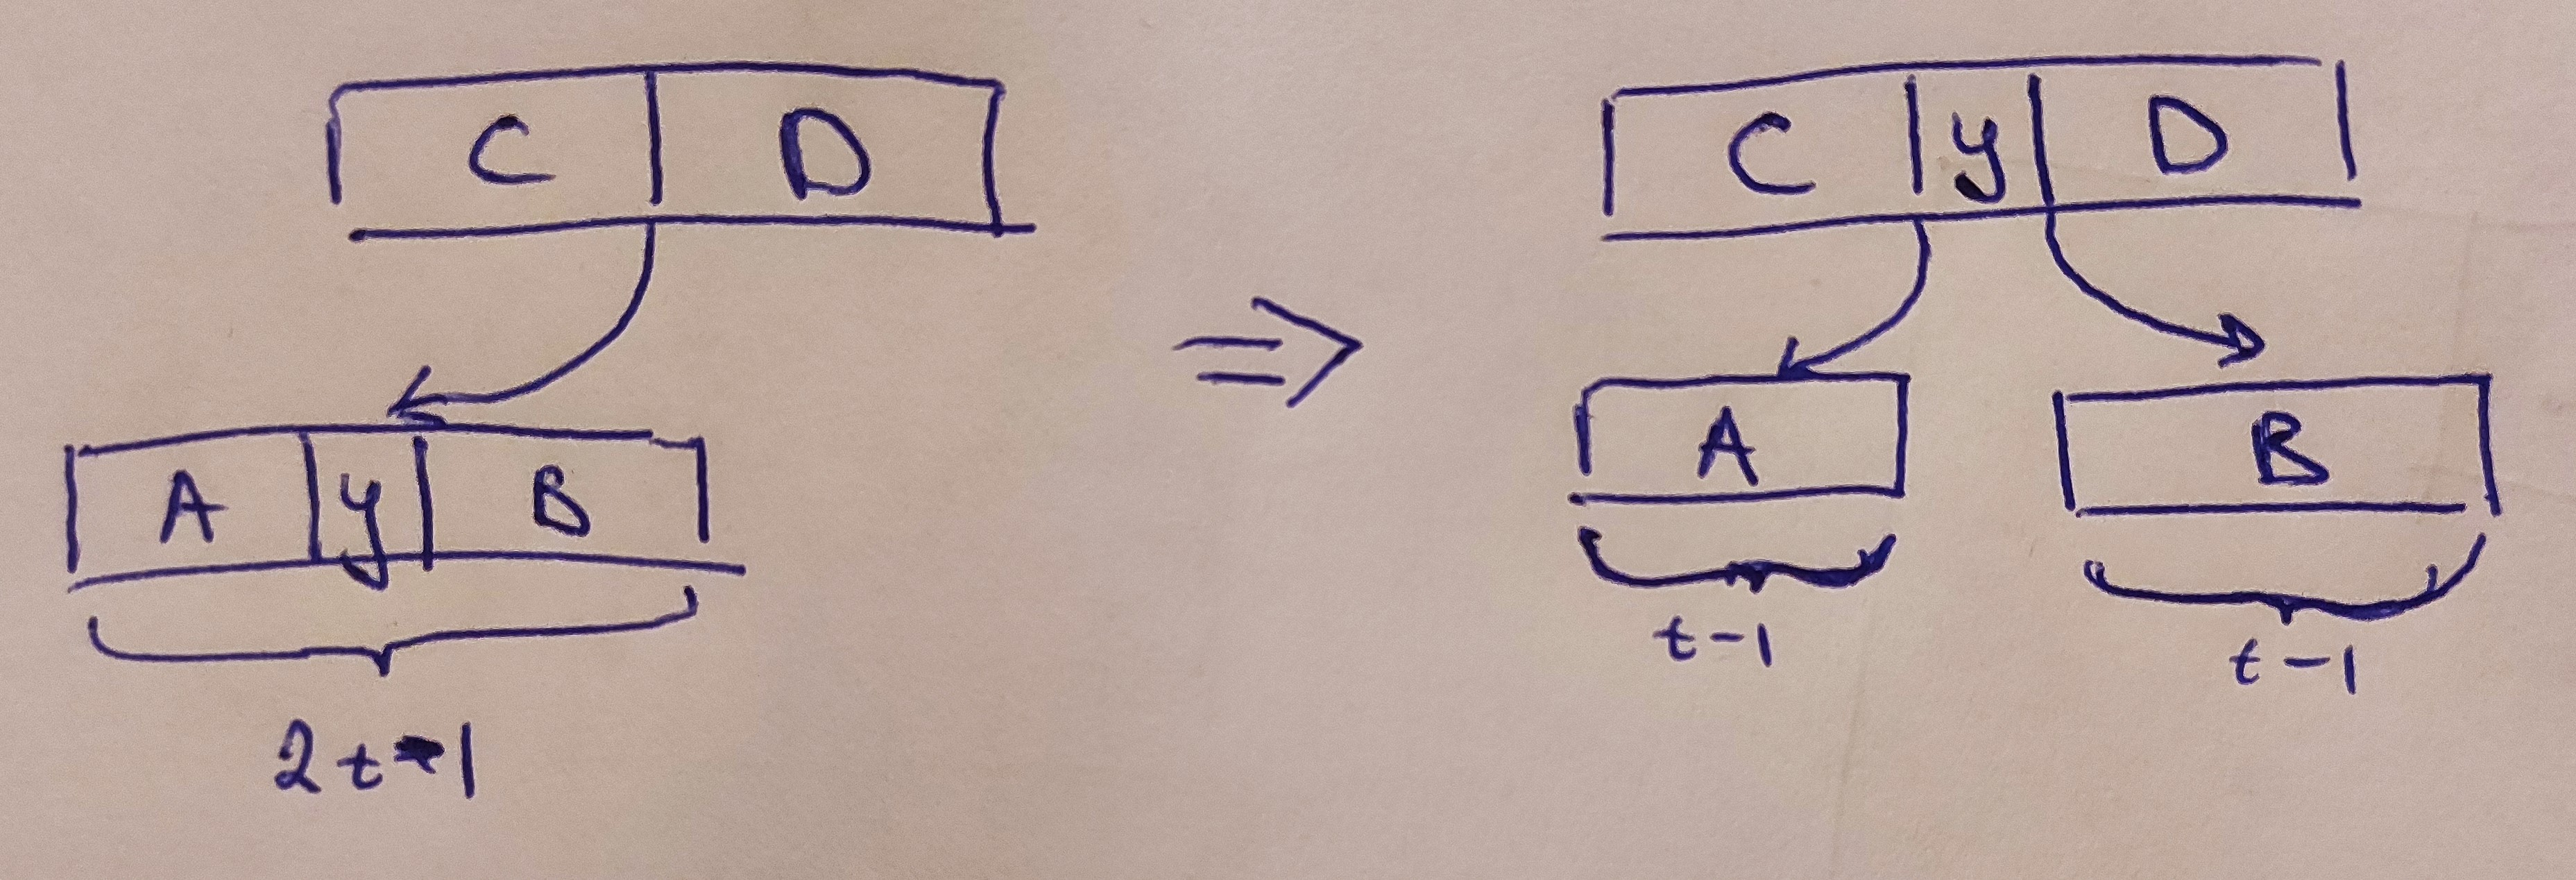
\includegraphics[scale=0.1]{images/51-54_b split.jpg}
\end{figure}
\par Добавление ключа в B-дереве может быть осуществлена за один нисходящий проход от корня к листу. Для этого не нужно выяснять, требуется ли разбить узел, в который должен вставляться новый ключ. При проходе от корня к листьям в поисках места для нового ключа будут разбиваться все заполненные узлы, которые будут пройдены (включая и сам лист). Таким образом, если надо разбить какой-то полный узел, гарантируется, что его родительский узел не будет заполнен.
\\

\setcounter{section}{53}
\section{Реализация операции erase в B-дереве.}
\par Поддерживаем, что в вершине $v$, в которой мы находимся $\geqslant t$ ключей (если это не корень). Действуем следующим образом \begin{enumerate}
    \item Если в правом брате $\geqslant t$ ключей, то выбираем его самый левый ключ (именно в вершине, а не во всем поддереве), ставим его на место родителя, а родителя делаем самым правым ключом $v$.
    \begin{figure}[h]
        \centering
        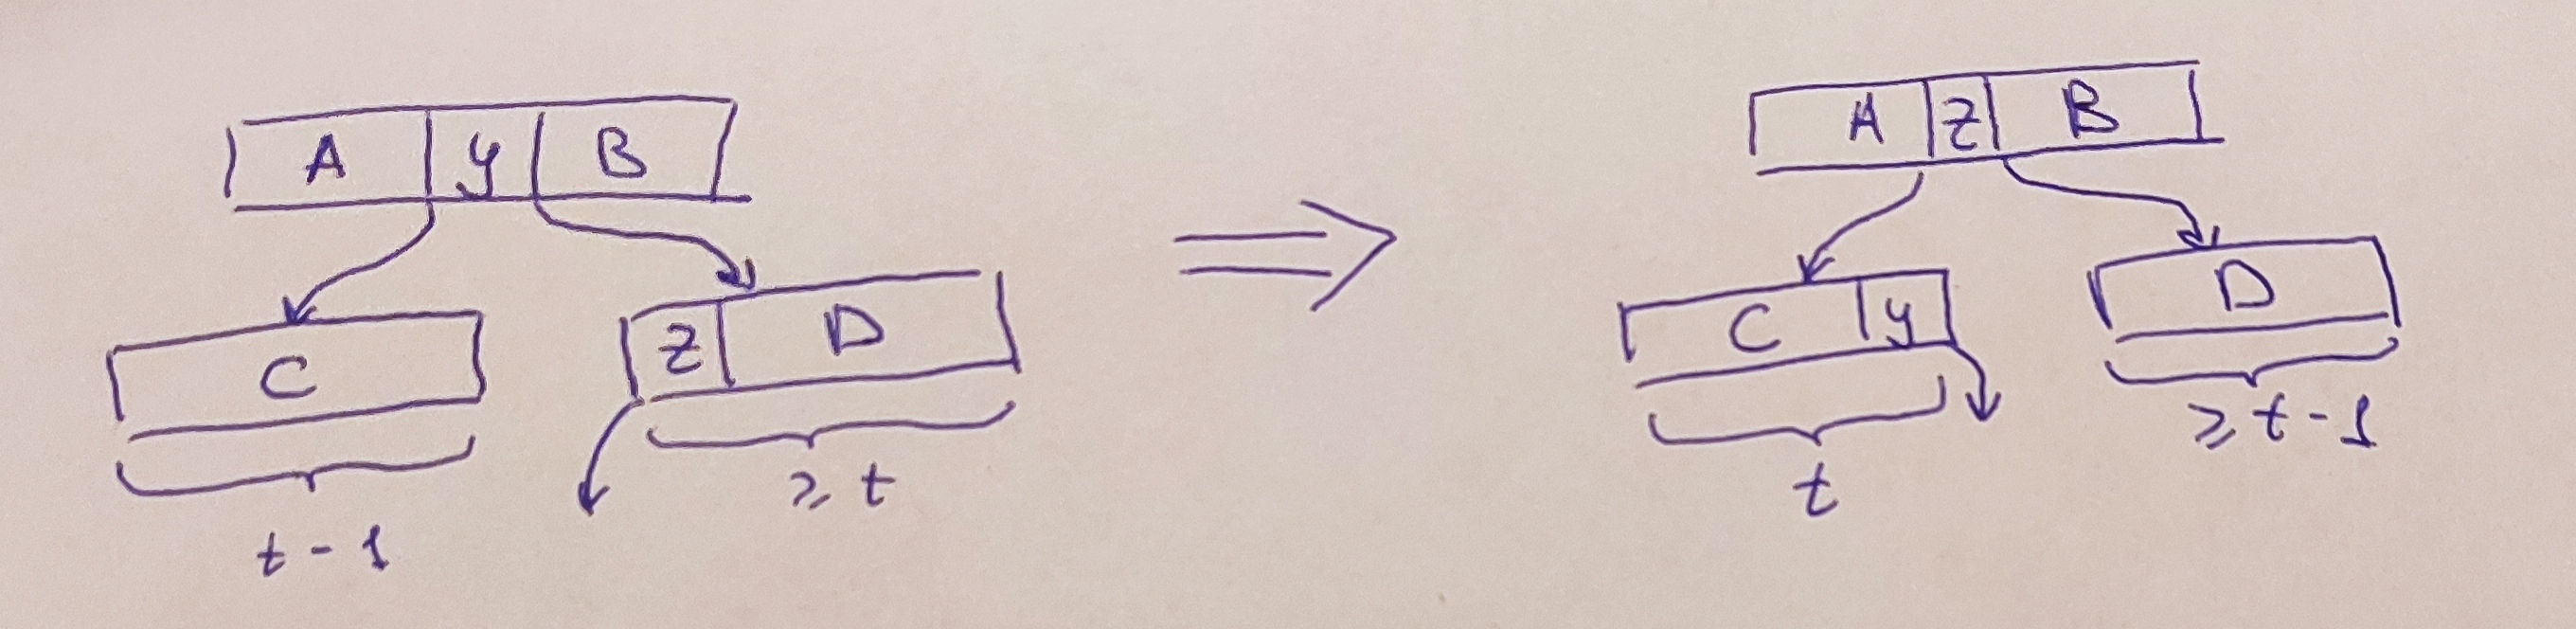
\includegraphics[scale=0.15]{images/51-54_b brothers.jpg}
    \end{figure}
    \item Если в левом брате $\geqslant t$ ключей, то делаем симметричные действия
    \item Если в обоих братьях $< t$ ключей, то объединяем $v$ с произвольным из них и спускаем родителя в объединенного ребенка (можем так сделать, так как в родительском узле $\geqslant t$ ключей)
    \begin{figure}[h]
        \centering
        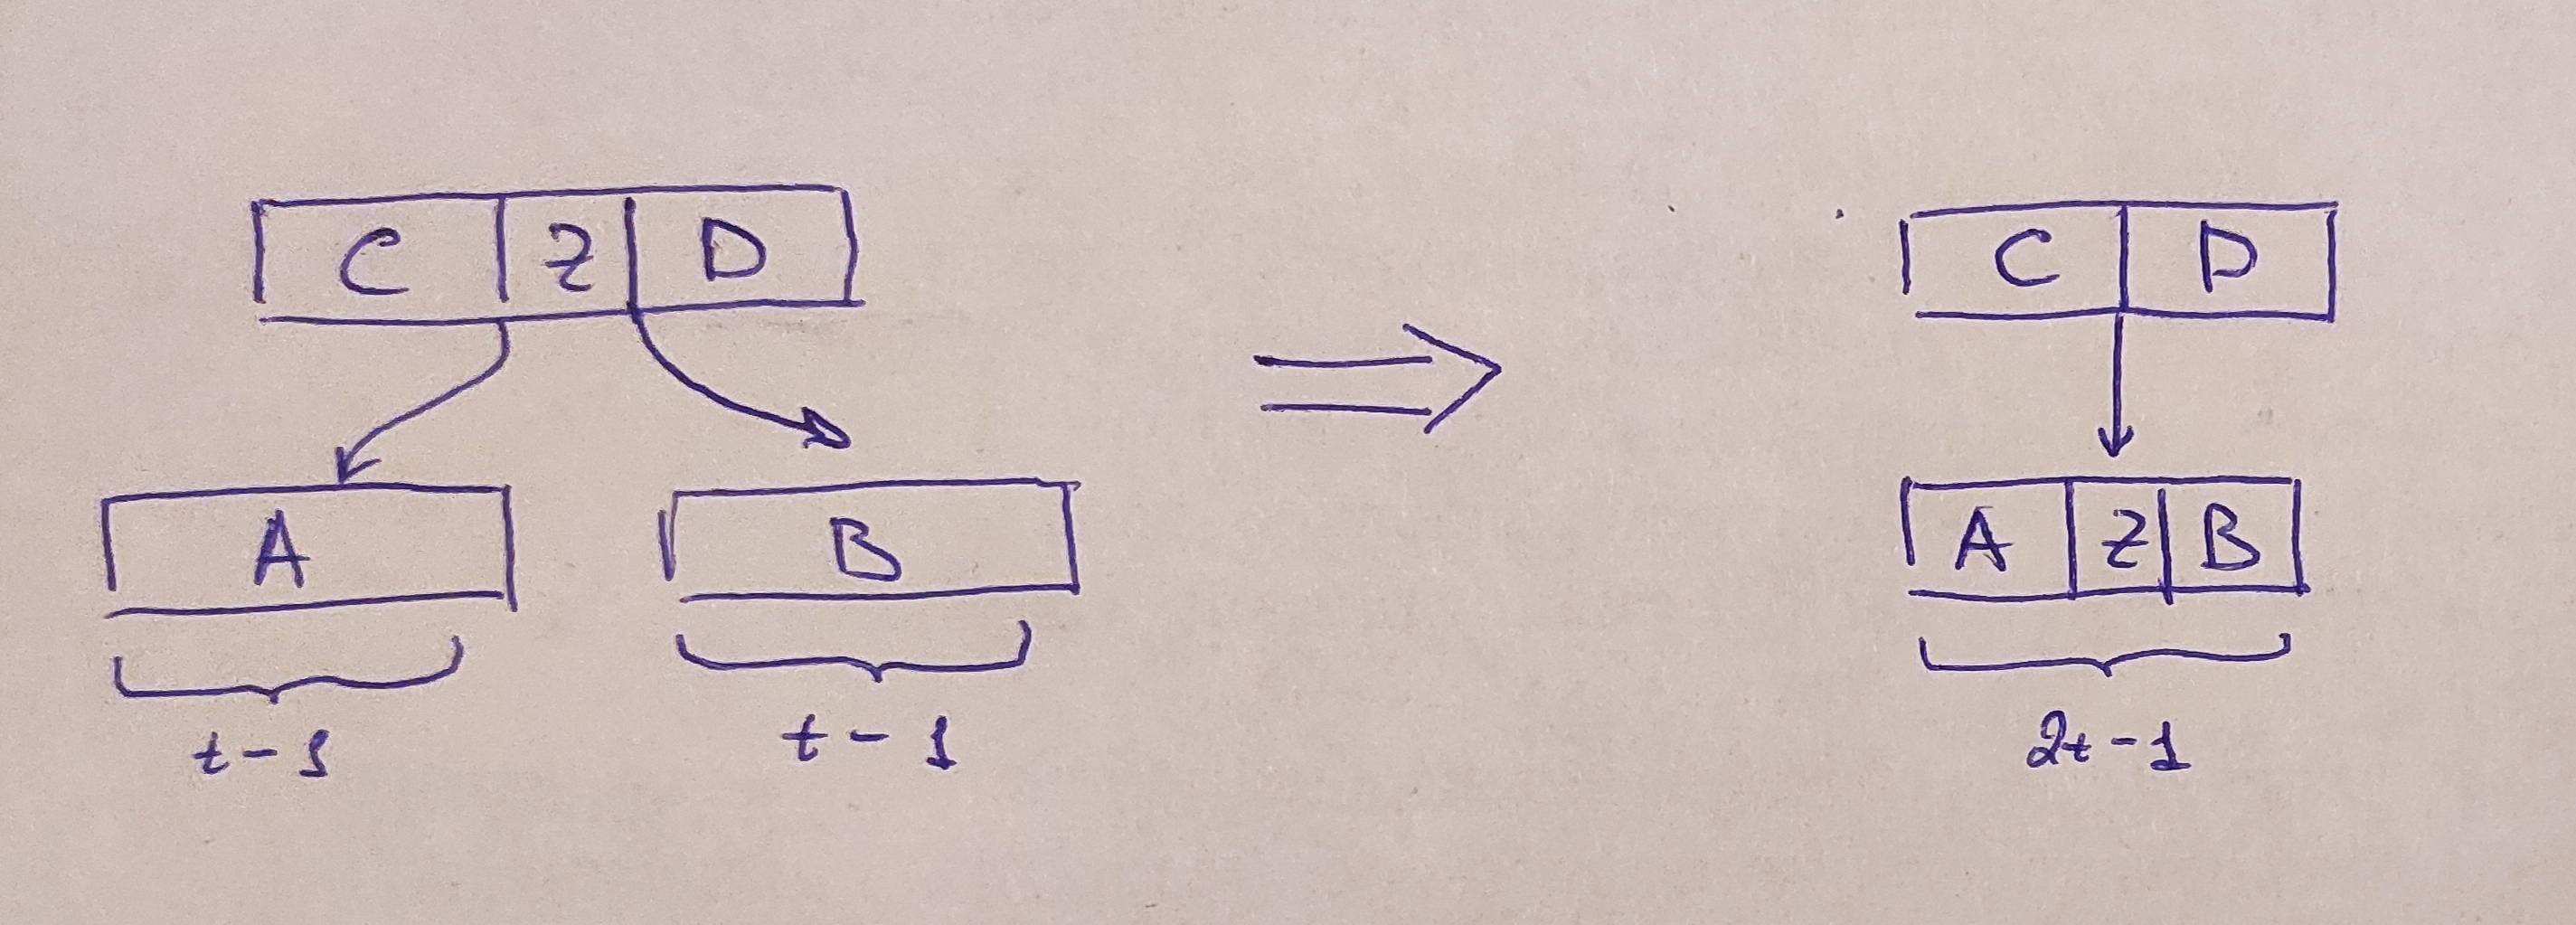
\includegraphics[scale=0.15]{images/51-54_b union.jpg}
    \end{figure}
\end{enumerate}
\par Если в какой-то момент мы переносим вниз последний ключ корня, то просто удаляем корень и делаем корнем его единственного сына.
\par Перейдем непосредственно к удалению. Находим $x$. 
\begin{enumerate}
    \item $x$ находится в листе, удаляем его. В листе точно осталось $\geqslant t-1$ ключей, то есть условие не нарушено 
    \item $x$ находится в нелистовой вершине \begin{enumerate}
        \item Если в левом сыне хотя бы $t$ ключей, то находим максимум в левом поддереве, удаляем его (так как он в листе можем воспользоваться пунктом 1) и ставим на место $x$.
        \item Если в правом сыне хотя бы $t$ ключей, то делаем аналогичные действия с правым поддеревом.
        \item Иначе объединяем детей, спускаем $x$ в объединенного ребенка и запускаемся от него рекурсивно
    \end{enumerate}
\end{enumerate}